%!TEX encoding = UTF-8 Unicode
\documentclass[12pt]{article} 
\usepackage[left=0.75in,top=20mm,right=0.75in,bottom=0.3in]{geometry} % Document margins
\usepackage{CJK}
\usepackage{graphicx}
\usepackage{mathtools}
\usepackage{mathrsfs}
\usepackage{amssymb}
\usepackage{hyperref}
\usepackage{sidecap}
\usepackage{makecell}
\usepackage{fancyhdr}

\fancypagestyle{title}{
  \setlength{\headheight}{15pt}
  \fancyhf{}
  \renewcommand{\headrulewidth}{0pt}
  \renewcommand{\footrulewidth}{0pt}
  \fancyhead[R]{Parallel Programming 2015}
}

\pagestyle{title}

\makeatletter
\renewenvironment{itemize}
{\list{$\bullet$}{\leftmargin\z@ \labelwidth\z@ \itemindent-\leftmargin
\let\makelabel\descriptionlabel}}
{\endlist}
\makeatother

\begin{CJK}{UTF8}{bsmi}
\title{\textbf{ Homework 3 / Mandelbrot set }}
\author{\textbf{李豪韋 (HW-Lee) ID 103061527}}
\date{}

\begin{document}
\vspace*{-60pt}
{\let\newpage\relax\maketitle}
\thispagestyle{title}

\section*{Overview}
\vspace{-20pt}
\noindent\makebox[\linewidth]{\rule{\textwidth}{0.4pt}}
\vspace{5pt}

Assumed that there is an infinite sequence $Z(c) = \{z_n|n \in \mathbb{N}\}$ that can be generated by a complex number $c$ with a recursive mapping $z_{n+1} = z_n^2 + c$ where $z_1 = c$, the Mandelbrot set is a set of complex numbers such that all elements in $Z(c)$ do not diverge to infinity. Mathematically, the Mandelbrot set can be defined as $\mathbb{M} = \{c|\displaystyle\lim_{n \to \infty}\|z_n(c)\| < \infty , c \in \mathbb{C}\}$, and it can be derived into the further form that we can obtain it more easily:
\begin{center}
    $\mathbb{M} = \{c|\displaystyle\lim_{n \to \infty}\|z_n(c)\| < 2 , c \in \mathbb{C}\}$
\end{center}

To implement a program that computes the Mandelbrot set in an numerical way, the complex space must be bounded by a specific rectangular and the sampling resolution must be designated. Moreover, we cannot check if the sequence remains a small enough norm with infinity, the maximum iteration number must be defined as well. In this way, the program will be able to obtain the Mandelbrot set by sampling points in the region and determining if the point belongs to the Mandelbrot set if $\|z(c)_{MAX_ITER}\| < 2$. For the convenience of discussing it in more detailed way, each point will be coloured with its iterations into gray-scaled. After all, the output image looks like below:

\begin{center}
    \begin{SCfigure}[][h]
        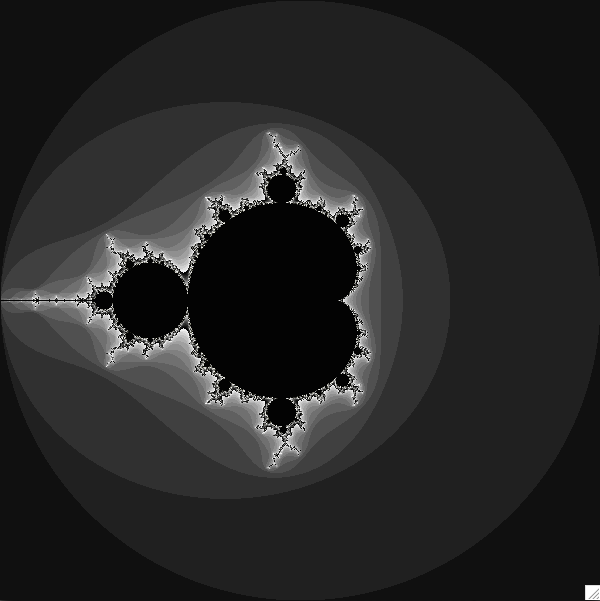
\includegraphics[scale=.5]{./coloring_ta.png}
        \caption{An example showing the Mandelbrot set where the points are ranged from $(-2, -2)$ to $(2, 2)$. Note that the brightness does not directly refer to the magnitude, the raw iterations are processed with modulo function to pronounce the difference between each pair of adjacent region. Therefore, we can observe the 'transition' between adjacent regions easily. However, I think this coloring method is not such good and the coloring methods I use will be discussed in the following section.}
    \end{SCfigure}
\end{center}

\newpage

Obviously, it is important to decide the strategy separating jobs. Because the number of iterations of the point seems to be subjected to the distance from the origin rather than the position, simply deviding the data into a couple of equally large subsets might induce a bad speedup performance due to the unbalanced loads among workers. Therefore, the project is aimed at making us get familiar with APIs and analyze/fine tune a better scheduling strategy.

\section*{Implementation}
\vspace{-20pt}
\noindent\makebox[\linewidth]{\rule{\textwidth}{0.4pt}}
\vspace{5pt}

In the project, the program is implemented with three different APIs, MPI/OpenMP/Hybrid, and two different scheduling strategies, static/dynamic.

\begin{itemize}
    \item Static scheduling: each worker processes same number of columns.
    \vspace{-.5cm}
    \begin{SCfigure}[][h]
        \hspace{-1cm}
        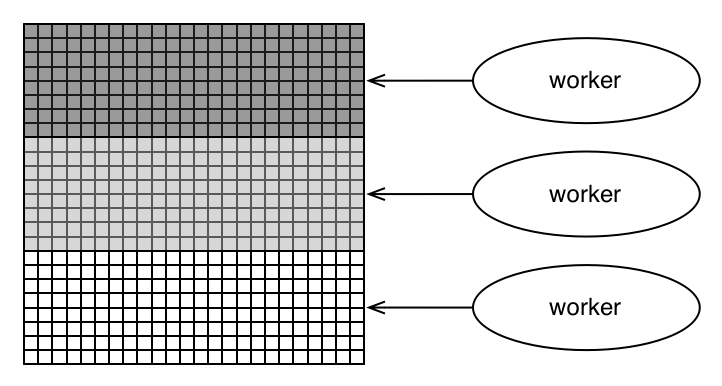
\includegraphics[scale=.5]{./flow_chart_static.png}
        \hspace{-.5cm}
        \vspace{-2cm}
        \caption{Static scheduling: the whole data will be equally separated into several pieces and each work processes its own piece.}
    \end{SCfigure}
    \vspace{1cm}
    \item Dynamic scheduling: each column is assigned dynamically to the worker which completes its task.
    \vspace{-.5cm}
    \begin{SCfigure}[][h]
        \hspace{-1cm}
        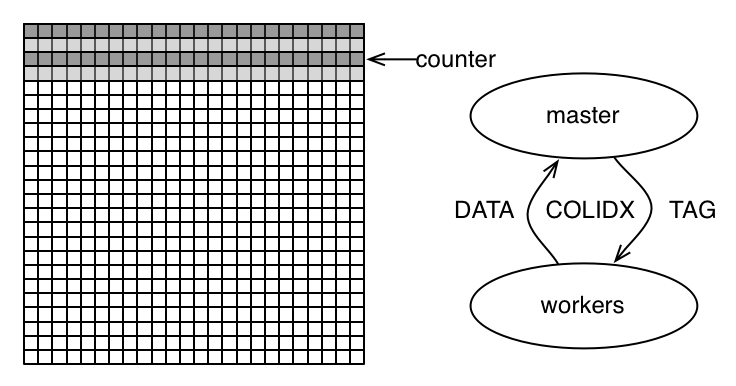
\includegraphics[scale=.5]{./flow_chart_dynamic.png}
        \hspace{-.5cm}
        \vspace{-.5cm}
        \caption{Dynamic scheduling: Only a small batch of columns are assigned to specific workers at the begining, and there is a master that monitors if each worker completes its job and then sends the next job and increments the counter until there is no job remains in the queue. This way provides a more flexible assigning strategy that keeps all workers work during the program.}
    \end{SCfigure}
\end{itemize}

\newpage

\section*{Analysis \& Results}
\vspace{-20pt}
\noindent\makebox[\linewidth]{\rule{\textwidth}{0.4pt}}

\section*{Discussion}
\vspace{-20pt}
\noindent\makebox[\linewidth]{\rule{\textwidth}{0.4pt}}

\end{CJK}
\end{document}